% !TEX ROOT = ../ersti.tex
\section{Überblick}
\label{hopo}
\marginpar{
    \centering{
        \vspace{2mm}
        
\includegraphics[width=3cm]{bilder/duty_calls.png}\\\vspace{5mm}
    }
}

Die Hochschulpolitik befasst sich mit allen politischen Vorgängen
bezüglich der Hochschulen in Deutschland. Dies beinhaltet Abläufe in den
Landes"= und Bundesparlamenten, den Gremien der universitären
Selbstverwaltung und der Öffentlichkeit. Thematisch umfasst die
Hochschulpolitik unter anderem den Bau, die Finanzierung, den rechtlichen
Status der Hochschulen, den Rahmen für Forschung und Lehre, aber auch die
soziale Stellung der Studierenden.

So wird über Studien"= und Prüfungsordnung, Organisation, Gliederung und
Ausrichtung der Hochschulen weitestgehend vor Ort entschieden, während
andere Entscheidungen die Kompetenz der Universität übersteigen. Sehr
deutlich wird dies bei den Regelungen über das BAföG
(Bundes"=Ausbildungsförderungs"=Gesetz), Wohnheimmieten oder kommunale
Verkehrspolitik (Fahrradwege, Semesterticket, \dots).

Die studentischen Belange werden bei der Entscheidungsfindung leider
häufig nur unzureichend berücksichtigt. Eine Ursache hierfür ist durch das
Hochschulrecht gegeben, welches den Studierenden nur eine bescheidene
Mitwirkung in den offiziellen Gremien der Universität zugesteht. Eine
Mitarbeit in anderen Gremien der Bildungslandschaft ist überhaupt nicht
vorgesehen. Natürlich gibt es Überschneidungen zwischen den Interessen der
Studierenden und denen des Landes bzw. des Bundes als Träger und
Finanziers der Hochschulen im Großen sowie zwischen den Studierenden und
den ProfessorInnen vor Ort. Die Entscheidungen, die in den letzten Jahren im
Bereich der Hochschule getroffen wurde, lassen allerdings deutlich
erkennen, dass diese Interessen im Vergleich zum Sparwillen der
öffentlichen Kassen nur geringe Priorität besaßen.

Ein weiterer Grund für die vergleichsweise geringe Beachtung der
Studierenden in Entscheidungsfindungsprozessen ist deren Situation und
sozialer Status. Zum einen sind die Studierenden keine homogene Gruppe:
Die einen finanzieren sich ihr Studium selbst, während andere durch ihre
Eltern unterstützt werden -- wieder andere werden von
einer Stiftung gefördert. Andererseits ist die Studienzeit gewöhnlich nur
ein auf politischer Skala kurzer Lebensabschnitt, der nach wenigen Jahren
wieder beendet ist. Die Wirkung von heute beschlossenen, politischen
Entscheidungen betrifft in den meisten Fällen erst die Studierenden von
morgen.

Umso wichtiger ist die studentische Mitwirkung aus eigenem Engagement. Der
folgende Artikel stellt den institutionellen Rahmen dar, in dem sich
politische Arbeit von Studierenden an der Universität und darüber hinaus
bewegt.

\subsection{Gesetzlicher Rahmen}
Grundsätzlich ist Hochschulrecht Landesrecht. Der Bund gab lange Zeit im
Hochschulrahmengesetz (HRG) Vorgaben, die im Landesrecht ausgestaltet
wurden. Am 26. Januar 2006 wurde vor dem Bundesverfassungsgericht (BVG)
ein Kompetenzstreit über die Zuständigkeit in der Hochschulpolitik
zwischen dem Bund und den Bundesländern Baden"=Württemberg, Bayern, dem
Saarland, Sachsen, Sachsen"=Anhalt und Hamburg geklärt. Der Bundestag hatte
in der 6. Novelle des Hochschulrahmengesetzes ein „in der Regel
gebührenfreies Erststudium“ verlangt und die Einführung von Verfassten
Studierendenschaften zwingend vorgeschrieben. (Die Verfassten
Studierendenschaften werden im Laufe dieses Artikels noch besprochen.) Das
Verfassungsgericht stellte fest, dass der Bund in diesen Fragen solange
nicht zuständig ist, bis die Notwendigkeit einer einheitlichen Regelung
für die Herstellung gleicher Lebensverhältnisse in den verschiedenen
Ländern nachgewiesen wurde. Die Fragestellung, ob eventuell einzuführende
Studiengebühren der Verfassung entsprechen, wurde dabei nicht verhandelt.
Seit der Förderalismusreform im Jahr 2006 ist die Gesetzgebungskompetenz
vollständig auf die Länder übergegangen. Der Bund ist lediglich indirekt
z.B. über das BAföG (Bundesausbildungsförderungsgesetz) oder
Forschungsförderungsprojekte (z.B. die Exzellenzinitiative) eingebunden.
Amtierende Ministerin auf Bundesebene ist \wissenschaftsministerbund.


Die Wissenschaftsministerin in Baden"=Württemberg ist zur Zeit \wissenschaftsministerbawue.
Das wesentliche Landesgesetz für die Form der
baden"=württembergischen Hochschulen wurde durch das seit 1. Januar 2000
geltende Universitätsgesetz (UG) bestimmt. Am 9. Dezember 2004
verabschiedete der Landtag von Baden"=Württemberg ein neues
Landeshochschulgesetz (LHG), das insbesondere Änderungen in der
Kompetenzverteilung zwischen den Gremien der universitären
Selbstverwaltung vorsah. Ziel schien dabei zu sein, Kompetenzen weg von
Gremien hin zu Einzelpersonen zu verlagern. So wurden dem Senat, dem
traditionellen akademischen Entscheidungsgremium der Universität (mit
Mitgliedern aller Gruppen und Fakultäten) zahlreiche Kompetenzen genommen
und auf das Rektorat übertragen. Genaueres zu den Gremien der Universität
und ihrer Verflechtung erfahrt ihr weiter unten. Die Möglichkeiten des
Wissenschaftsministeriums, auf die Besetzung der Position des Rektors und
die Zusammensetzung des Aufsichtsrates einzuwirken, wurden gesteigert.

Die aktuelle grün-rote Landesregierung hat eine Novelle des LHGs ausgearbeitet, 
die am 27.03.2014 als „Drittes Hochschulrechtsänderungsgesetz“ beschlossen wurde.
Inwiefern sich die dortigen Änderungen konkret auf den Alltag an den Universitäten 
auswirken werden, wir abzuwarten sein.


\subsection{Aus der jüngsten Geschichte der Mitbestimmung an den Hochschulen}
%\mathphyssecnobar{Aus der jüngsten Geschichte der Mitbestimmung an den Hochschulen}

\sidebar{
    \centering
    
\includegraphics[width=3cm]{bilder/dear_CERN_1.png}\\\vspace{14mm}
    
\includegraphics[width=3cm]{bilder/dear_CERN_2.png}\\\vspace{14mm}
    
\includegraphics[width=3cm]{bilder/dear_CERN_3.png}\\\vspace{14mm}
    
\includegraphics[width=3cm]{bilder/dear_CERN_4.png}\\\vspace{14mm}
    
\includegraphics[width=3cm]{bilder/dear_CERN_5.png}\\\vspace{14mm}
    
\includegraphics[width=3cm]{bilder/dear_CERN_6.png}
}

Bis 1969 hatten die LehrstuhlinhaberInnen (Ordinarien) das Sagen an den
Universitäten. Sie hatten praktisch die alleinige Entscheidungsbefugnis
für ihrenjeweiligen Lehr"= und Forschungsbereich. Sämtliche Gremien setzten
sich alleine aus LehrstuhlinhaberInnen zusammen. 1969 wurde diese
Ordinarienuniversität im Zuge der Forderungen nach Demokratisierung und
Mitbestimmung abgeschafft und die Gruppenuniversität eingeführt. Die
Mitglieder der Universität wurden in Gruppen eingeteilt, die
ProfessorInnen, die wissenschaftlichen MitarbeiterInnen (=\ Mittelbau), die
StudentInnen sowie die sonstigen MitarbeiterInnen (=\ Sonstige). Jeder
dieser „Stände“ wählt bei Uniwahlen eine bestimmte Anzahl VertreterInnen
in die Gremien der Uni. Der „erste Stand“, die ProfessorInnen, stellen
zusätzlich eine gewisse Anzahl von Mitgliedern kraft Amtes. Für eine kurze
Phase wählten alle Gruppen außer den Sonstigen (HausmeisterInnen,
SekretärInnen, \dots) gleich viele VertreterInnen („Drittelparität“).
1973 stellte das Bundesverfassungsgericht (mit 6:2 Stimmen) aber fest, dass
aufgrund der grundgesetzlich garantierten Freiheit von Forschung und Lehre
(Art. 5 GG) die Gruppe der ProfessorInnen in allen Gremien eine
maßgebende, bzw. in bestimmten Fragen eine ausschlaggebende Mehrheit haben
muss. Damit ist eine relative bzw. in einigen Gremien eine absolute
Mehrheit gemeint. Aufgrund dieses Urteils sind die Entscheidungsgremien so
zusammengesetzt, dass ProfessorInnen mindestens so viele Sitze haben wie
alle anderen Gruppen zusammen.



\section{Studentische Vertretung}
Um die Interessen der Studierenden artikulieren und durchsetzen zu können,
muss es eine Instanz geben, die sie vertritt. In einigen Bundesländern
(ab 01. Januar 2013 allen außer Bayern) nimmt diese Aufgabe die
Verfasste Studierendenschaft (VS) war, d.h. die Studierenden geben sich
in eine Vertretung, meistens einen Studierendenrat (StuRa)
oder auch ein Studierendenparlament, der/das eine „Regierung“, den AStA
(Allgemeiner Studierendenausschuß) wählt, welcher die Beschlüsse der VS
vollzieht und z.B. über die zur Verfügung stehenden Finanzen beschließt.
Die Rechte der Verfassten Studierendenschaft können dabei sogar so weit
reichen, dass diese als Gemeinschaft öffentlichen Rechtes eigene Verträge
abschließen kann -- oft basieren Semestertickets auf solchen Verträgen.

In Baden"=Württemberg gab es schon einemal (bis 1977) eine Verfasste
Studierendenschaft. Um die Studierenden vor politischen Dummheiten zu
bewahren, wurde jedoch 1977 - als weitere Folge des Urteils von 1973 - in
den Ländern Bayern und Baden"=Württemberg die VS in der bisherigen Form
vorsichtshalber abgeschafft. Da es aber einem demokratischen Staat mit
folglich demokratischen Universitäten wiedersprach, wenn die
zahlenmäßig stärkste Gruppe ausgeschaltet wird, richtete man einen
besonderen Ausschuss des Senats ein: den Ausschuss für musische,
sportliche, geistige und soziale Belange der Studierenden. Diesen rein
beratenden Ausschuss bezeichnete man einfach genauso wie die bisherige
Studierendenvertretung als AStA (im folgenden nur noch als sogenannter
AStA, „AStA“ bezeichnet). Er wird gebildet aus den studentischen
Mitgliedern des Senats und einigen KandidatInnen entsprechend der
erhaltenen Stimmenanzahl. Tätig werden durfte der baden"=württembergische
Pseudo-„AStA“ gemäß LHG nur unter der Rechtsaufsicht des Rektors. Zu
Fragen des Studiums, zu Problemen einzelner Fachbereiche oder gar zu
politischen Fragen, z.B. BAföG oder Semesterticket darf der „AStA“ nicht
aktiv werden. Eine Vertretung auf Fachbereichsebene war überhaupt nicht
vorgesehen.

Auf diese Beschneidung ihrer Rechte reagierten die
Studierenden, indem sie ihre eigenen Vertretungen parallel zur
Pseudovertretung im „AStA“ schufen. Im Gegensatz zu den abhängigen,
offiziellen Gremien wurden sie als unabhängige Gremien bezeichnet.
An vielen Fachbereichen gibt es kontinuierlich oder immer mal wieder
Institutsgruppen, Fachschaftsinitiativen oder unabhängige Fachschaften,
die sich durch öffentliche Treffen und ihre Arbeit am Fachbereich
(Gremienarbeit, Klausurensammlung, Vorlesungsumfragen, Feten,
ErstsemesterInneneinführungen) legitimieren. Sie setzen sich vor Ort für
die Belange der Studierenden eines Faches ein. Diese Vertretungs"= und
Arbeitsstrukturen ersetzten wirkungsvoll die bisher fehlende gesetzlich verankerte
Mitbestimmung oder gar Vertretung. Wie die Zusammenarbeit mit den
jeweiligen Instituten oder Seminaren klappt, hängt jedoch immer noch vom
Wohlwollen der ProfessorInnen, des Rektors/der Rektorin und des Ministeriums ab. In den
Fachbereichen Mathematik, Physik und Informatik übernahm diese Aufgabe
seit 1983 die Fachschaft MathPhys\footnote{\url{http://mathphys.fsk.uni-heidelberg.de}}.
Im Zuge der Einführung der Verfassten Studierendenschaft (siehe folgender Absatz) hat sich der Zusammenschluss MathPhys
wieder in die drei Teilfachschaften Mathematik, Informatik und Physik aufgeteilt.
Das gemeinsame „Dach“ MathPhys ist aber erhalten geblieben, um fachschaftsübergreifende
Arbeit zu koordinieren und weiterhin einen kollegialen Austausch zu ermöglichen.


\subsection{Ein Klassiker kehrt zurück: die VS}

Mit dem „Gesetz zur Einführung einer Verfassten Studierendenschaft und
zur Stärkung der akademischen Weiterbildung
(Ver\-fass\-te-Stu\-dier\-en\-den\-schafts-Ge\-setz -- VerfStudG)“ hat der Landtag am 27. Juni 2012
die Wiedereinführung\footnote{Offiziell ist nur von der „Einführung“ die
Rede, da die neue VS nicht die offizielle Rechtsnachfolge der alten VS sein soll.
Grund ist, dass das Land andernfalls höhere Millionenbeträge zurückzahlen müsste,
die der VS 1977 enteignet wurden.} der Verfassten Studierendenschaft beschlossen.

Über die Form der Verfassten Studierendenschaft -- also die Frage, welche
Struktur die studentische Selbstverwaltung bekommen sollte -- haben die Studierenden
der Universität Heidelberg vom 13. bis 15. Mai 2013 per Urabstimmung abgestimmt.
Es standen zwei Modelle zur Auswahl: Ein Modell mit zwei
Kammern (Studierendenparlament und FSK) sowie ein Modell mit nur einer
Kammer (ein sog. Studierendenrat). Unsere Fachschaft hatte nach intensiven Diskussionen mit
VertreterInnen beider Initiativen einen eindeutigen
Konsens dahingehend gefunden, dass sowohl für unsere Studierenden aus
Mathe/Info/Physik/Astronomie, als auch für die Studierendenschaft
insgesamt das Zweikammernmodell deutlich größere Vorteile besitzt als
das Einkammernmodell\footnote{Wen unsere Gründe interessieren, sie sind in unserem FS-Info-Heft MPI 1-2013 nachlesbar}.
Bei der Urabstimmung hat sich allerdings die Mehrheit der Studierenden (58,87\%)
für das Einkammernmodell ausgesprochen, weshalb wir im Folgenden nur dieses Modell beschreiben.



\subsection{Die Gremien der VS}

Die Verfasste Studierendenschaft gliedert sich in Heidelberg in sogenannte
Studienfachschaften. Eine Studienfachschaft umfasst alle
Studierenden eines Faches, in eurem Fall gehört ihr also zu einer der
Studienfachschaften Informatik, Mathematik oder Physik\footnote{Falls ihr
mehr als ein Hauptfach studiert -- z.B. im Lehramtsstudiengang -- werdet
ihr standardmäßig der Studienfachschaft eures ersten Hauptfaches zugeordnet.
Sofern ihr in eurem zweiten Hauptfach wählen möchtet, müsstet ihr dorthin „optieren“.
Details hierzu findet ihr auf der Homepage des Wahlamts der Universität}.
Bitte prüft in der Zeit vom 11. bis 18. Oktober euren Eintrag im Wäherverzeichnis
(einsehbar auf der Homepage des Wahlamts). Sofern ihr dort nicht auftaucht,
dürft ihr bei der Wahl vom 18. bis 20. November nicht wählen.

Auf Ebene der Studienfachschaften gibt es zwei Organe: Eine „Vollversammlung“ 
(auch „Fachschaftssitzung“ genannt) und einen gewählten „Fachschaftsrat“. In den 
Fachschaften Informatik, Mathematik und Physik haben wir uns dafür entschieden, 
den Fachschaftsrat als lediglich ausführendes Organ zu gestalten, die 
Entscheidungskompetenzen liegen bei der regelmäßig statt findenden Fachschaftssitzung.
Das bedeutet, ihr könnt ohne euch extra wählen lassen zu müssen jederzeit
auf Fachschaftsebene mitarbeiten und mitentscheiden.

Auf zentraler Ebene gibt es in Heidelberg als legislatives Orgen den Studierendenrat (StuRa). 
Er besteht aus VertreterInnen aller Studienfachschaften, die von diesen entsandt werden
(ca. 64 Personen) sowie aus direkt durch die Studierenden gewählten Mitgliedern.
Die Anzahl der direkt gewählten Mitglieder skaliert mit der Wahlbeteiligung
und liegt zwischen 0 Personen (bei 0\% Wahlbeteiligung) und ebenfalls 64 Personen
(bei 50\% oder höherer Wahlbeteiligung).

Der Studierendenrat beschließt als zentrales legislatives Organ über alle
zentralen Belange der Studierendenschaft (Höhe der Beiträge, Finanzen,
Wahl der Referate, etc.).

Das exekutive Organ der VS ist in Heidelberg die sogenannte „Referatekonferenz“ sein.
Sie besteht aus vom Studierendenrat für bestimmte Aufgabenbereiche (z.B.
Kommunales, Ökologie, Hochschulpolitik, Soziales, \dots) gewählten
ReferentInnen. Diese setzen Beschlüsse des StuRa um und können sogar --
sofern der StuRa keine Entscheidung treffen kann oder (z.B. weil zu
wenige Mitglieder anwesend sind) nicht beschlussfähig ist --
eigenständig im Namen der Studierendenschaft entscheiden.

\subsection{Hintergründe zur VS}

\paragraph{Mitgliedschaft in der Verfassten Studierendenschaft}

Alle Studierenden sind qua Immatrikulation automatisch Mitglied der
Verfassten Studierendenschaft. Weil sie die einzige Möglichkeit zur
Partizipation an legitimierter Studierendenvertretung ist und ihre
Leistungen für alle Studierenden offen stehen müssen, ist ein Austritt
nicht möglich.

\paragraph{Rechtsfähigkeit}

Bisher ist der „AStA“ (Allgemeiner Studierendenausschuss) nur ein Ausschuss
im Gesamtgebilde Universität. Durch die Verfasste Studierendenschaft wird
die Studierendenvertretung zu einer eigenständigen, rechtsfähigen Teilkörperschaft
innerhalb der Universität. Dadurch kann sie selbst Verträge abschließen und
so z.B. mit den Verkehrsbetrieben direkt über das Semesterticket verhandeln
oder Leasing-Fahrzeuge vergünstigt an die Studierenden vermieten.
Diese Rechtsfähigkeit gilt allerdings nur für die VS als ganzes,
nicht für ihre Organe (z.B. Fachschaften).

\paragraph{Beitragshoheit}

Die VS kann von allen Studierenden Beiträge erheben, die zusammen mit dem
sonstigen Semesterbeitrag eingezogen werden. Mit der Einführung der VS
wurde leider nicht festgeschrieben, dass das bisherige von der Uni verwaltete
Budget des „AStA“, auf das die Studierendenvertretung zurückgreift,
bestehen bleibt. Die VS erhebt deshalb einen Beitrag von \EUR{7.50} pro 
Semester. Von diesem werden qua Satzung 40 Prozent an die dezentrale 
Studierendenvertretung durch Fachschaften fließen, der Rest wird auf zentraler, 
sprich universitätsweiter Ebene durch den StuRa verwaltet Damit soll nicht 
nur die schon vor Einführung der VS verrichtete Arbeit fortgeführt, sondern 
auch die Etablierung und Förderung neuer studentischer Projekte, besserer 
Kampagnen zur Vertretung derstudentischen Interessen und mehr Service ermöglicht 
werden.

\paragraph{Mandat}

Früher war der offizielle „AStA“, also der Senatsausschuss mit 11 gewählten
Mitgliedern, mit einem sportlichen, kulturellen, musischen und eingeschränkt
sozialen Mandat ausgestattet.
Mit dem Gesetz erhält die neue VS zusätzlich zu den alten Kompetenzen ein
hochschulpolitisches und soziales Mandat; sie darf sich außerdem zum Wirken
der Hochschule in der Gesellschaft äußern, z.B. durch Technikfolgenabschätzung,
sowie die politische Bildung der Studierenden fördern. In diesem Sinne hat
sie ein politisches Mandat. Dabei ist sie an das übliche Neutralitätsgebot
für staatliche Organe mit Pflichtmitgliedschaft gebunden, darf also z.B.
keine Werbung für religiöse oder parteipolitische Strukturen machen.

\section{Entscheidungsgremien der Universität}
Die Universität Heidelberg ist eine Lehr"= und Forschungseinrichtung mit
über 500 ProfessorInnen, circa 31\,000 Studierenden und vielen sonstigen
MitarbeiterInnen. Der Etat der Universität beträgt um die 620 Millionen
Euro. Die Aufgabe der Universität, die „Pflege und Entwicklung der
Wissenschaften und der Künste durch Forschung, Lehre und Studium“ (§2
% Quelle: http://www.umwelt-online.de/recht/allgemei/laender/bw/hschg01.htm
LHG), stellt hohe finanzielle und organisatorische Ansprüche.
Entscheidungen für die gesamte Hochschule treffen die zentralen Gremien,
Rektorat, Senat und Universitätsrat. Der Senat beschließt über
universitätsweite Belange wie Verlegung der Semesterzeiten, die
Immatrikulationsordnung und generell über grundlegende Fragen, welche die
Gesamtuniversität betreffen. Der Senat bestätigt Vorschläge der einzelnen
Fachbereiche über die Berufung neuer Professoren, genehmigt Lehrpläne und
beschließt über die Einrichtung oder Aufhebung von Studiengängen. Dem
Senat gehören außer dem Rektorat alle DekanInnen (das sind die
Vorsitzenden der Fakultäten), die Frauenbeauftragte und 8 gewählte
ProfessorInnen, 4 Studierende, 4 VertreterInnen aus dem Mittelbau und 4
Sonstige an. Das macht also ein Verhältnis von 27, bzw. 28 Profs gegen 12
andere, davon 4 Studis. Besondere Themen wie Umweltfragen oder
Prüfungsangelegenheiten werden in beratenden Ausschüssen des Senats
vorbereitet, in denen alle Gruppen vertreten sind, die ProfessorInnen
natürlich mit absoluter Mehrheit.

\sidebar{
    \centering
    
\includegraphics[width=3cm]{bilder/inequivalence_principle_1.png}\\\vspace{13mm}
    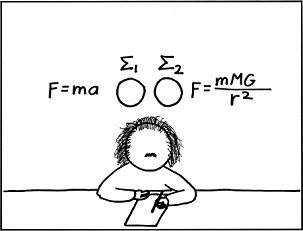
\includegraphics[width=3cm]{bilder/inequivalence_principle_2.png}\\\vspace{13mm}
    
\includegraphics[width=3cm]{bilder/inequivalence_principle_3.png}\\\vspace{13mm}
    
\includegraphics[width=3cm]{bilder/inequivalence_principle_4.png}\\\vspace{13mm}
    
\includegraphics[width=3cm]{bilder/inequivalence_principle_5.png}\\\vspace{13mm}
    
\includegraphics[width=3cm]{bilder/inequivalence_principle_6.png}
}


Den Universitätsrat gibt es erst seit dem Wintersemester 2000/2001. Er ist
eine Art Aufsichtsrat der Universität. Er berät über die strukturelle
Ausrichtung der Universität und hat das letzte Wort in
Finanzangelegenheiten. Er besitzt damit wesentlichen Einfluss auf die
künftige Entwicklung der Universität. 6 der 11 Mitglieder sind
Universitätsexterne aus Politik, Kultur und Wirtschaft, 5 Mitglieder
kommen aus der Universität. Alle Mitglieder werden vom
Wissenschaftsministerium benannt. Im Zuge der Novelle des LHG 2014 wurde
der Universitätsrat mit weiteren Kompetenzen ausgestattet.

Sieht man den Universitätsrat als Aufsichtsrat der Universität, wird das
Rektorat zum zugehörigen Vorstand. Es besteht aus dem/der RektorIn, 4
ProrektorInnen und dem/der LeiterIn der Verwaltung: dem/der KanzlerIn.
Rektor ist zur Zeit \rektor . Neben seinen Verwaltungsaufgaben in
der Uni, vertritt er sie auch nach außen, z.B. gegenüber dem Land. Das
Rektorat residiert in der alten Universität, Grabengasse 1. Die
Universitätsverwaltung ist in der Seminarstr. 2 angesiedelt.

\subsection{Die Fakultät}

Die speziellen Fragen eines Fachbereichs werden in der Fakultät, der
„organisatorischen Grundeinheit der Universität“, die „gleiche oder
verwandte Fachbereiche zusammenfasst“ (LHG), (vor)entschieden. Die
Universität Heidelberg ist in zwölf Fakultäten gegliedert, zum Beispiel 
die Fakultät für Mathematik und Informatik und die Fakultät für Physik und 
Astronomie. Während man an einigen Fakultäten nur ein bzw. wenige Fächer studieren
kann, gibt es andere Fakultäten, wie z.B. die Neuphilologische Fakultät,
an denen viele Fächer (Germanistik, Anglistik, Romanistik etc.) studiert
werden können. Geleitet wird die Fakultät von einem/einer DekanIn und dem
ihm unterstehenden Dekanat, das die laufenden Geschäfte erledigt. Der/Die
DekanIn wird für vier Jahre vom Fakultätsrat gewählt. Zur Zeit ist Dekan der
Mathematik Prof. \dekanmathe{} und in der Physik Prof. \dekanphysik. Zusammen mit dem
Studiendekan (s.u.) bilden Dekan und Prodekan den Fakultätsvorstand. Zu
finden ist das Dekanat der Mathe \gls{INF} 288, Zimmer 277 und das der Physik
INF 226, 2.OG.

Die Mitglieder der Fakultäten wählen in dem beschriebenen
Vierklassenwahlrecht den Fakultätsrat, das oberste Gremium der Fakultät.
Er ist zuständig für alle Fragen der Lehre und der Forschung. Ihm gehören
6 gewählte Profs, 5 Studierende, 4 Angehörige aus dem Mittelbau und 1 Mitglied
aus der Gruppe der MitarbeiterInnen aus Administration und Technik
an, außerdem alle InstitutsdirektorInnen und der Fakultätsvorstand, also Dekan,
Prodekan und Studiendekan. Abweichend davon kann sich eine Fakultät auch für einen
sogenannten „großen Fakultätsrat“ entscheiden (so geschehen beispielsweise in der 
Fakultät für Physik und Astronomie), in dem alle ProfessorInnen der Fakultät 
Mitglied sind. Die Mitgliederanzahlen der anderen Gruppen werden dabei ebenfalls
(leicht) erhöht. Der Fakultätsrat bildet Ausschüsse mit vergleichbarer
Zusammensetzung, die sich um bestimmte Bereiche kümmern, besonders wichtig
sind zum Beispiel die Prüfungsausschüsse oder die Studienkommissionen. Die
Mitglieder der Ausschüsse müssen nicht immer Mitglieder des Fakultätsrats
sein. Die Fakultäten gliedern sich weiter in Institute. Jedes Institut
wird von einem Institutsdirektor geleitet.

\subsection{StudiendekanIn und Studienkommission}

Mit dem Universtätsgesetz von 1995 wurde ein weiteres Gremium auf Fakultätsebene 
eingeführt: die Studienkommission. Diese ist ein Gremium, das den Studiendekan/die
StudiendekanIn, der/die Kraft Amtes ihr Vorsitzender/ihre Vorsitzende ist, berät.
StudiendekanIn und Studienkommission sollen gemeinsam zur Verbesserung der Lehre
beitragen. Die Studienkommission besteht aus StudiendekanIn, drei weiteren
ProfessorInnen, zwei VertreterInnen des Mittelbaus sowie vier Studierenden.
Hauptaufgaben der Kommission sind:
\begin{itemize}
    \addtolength{\itemsep}{-0.7\baselineskip}
    \item Empfehlungen zur Weiterentwicklung von Gegenständen und Formen des Studiums
    \item „Verfahren zur Bewertung und Verbesserung  der Qualität der Lehre unter
          Einbeziehung studentischer Veranstaltungskritik“ zu entwickeln
    \item In regelmäßigen Abständen einen Lehrbericht zu verfassen.
\end{itemize}

Die Umsetzung von Empfehlungen und die Wahrnehmung laufender Aufgaben
obliegt dem Studiendekan/der Studiendekanin. Die Kommission ist nur
beratend und die Durchsetzung ihrer Beschlüsse und Ideen ist vom guten
Willen des Fakultätsrats abhängig. Der Studiendekan / die Studiendekanin
nimmt die mit Forschung und Lehre zusammenhängenden laufenden Aufgaben
wahr; seine/ihre Aufgabe ist es insbesondere, auf ein ordnungsgemäßes und
vollständiges Lehrangebot hinzuwirken und die Beschlussfassung über
Studienpläne, Studien"= und Prüfungsordnungen und Lehrberichte
vorzubereiten.


